\documentclass[1p]{elsarticle_modified}
%\bibliographystyle{elsarticle-num}

%\usepackage[colorlinks]{hyperref}
%\usepackage{abbrmath_seonhwa} %\Abb, \Ascr, \Acal ,\Abf, \Afrak
\usepackage{amsfonts}
\usepackage{amssymb}
\usepackage{amsmath}
\usepackage{amsthm}
\usepackage{scalefnt}
\usepackage{amsbsy}
\usepackage{kotex}
\usepackage{caption}
\usepackage{subfig}
\usepackage{color}
\usepackage{graphicx}
\usepackage{xcolor} %% white, black, red, green, blue, cyan, magenta, yellow
\usepackage{float}
\usepackage{setspace}
\usepackage{hyperref}

\usepackage{tikz}
\usetikzlibrary{arrows}

\usepackage{multirow}
\usepackage{array} % fixed length table
\usepackage{hhline}

%%%%%%%%%%%%%%%%%%%%%
\makeatletter
\renewcommand*\env@matrix[1][\arraystretch]{%
	\edef\arraystretch{#1}%
	\hskip -\arraycolsep
	\let\@ifnextchar\new@ifnextchar
	\array{*\c@MaxMatrixCols c}}
\makeatother %https://tex.stackexchange.com/questions/14071/how-can-i-increase-the-line-spacing-in-a-matrix
%%%%%%%%%%%%%%%

\usepackage[normalem]{ulem}

\newcommand{\msout}[1]{\ifmmode\text{\sout{\ensuremath{#1}}}\else\sout{#1}\fi}
%SOURCE: \msout is \stkout macro in https://tex.stackexchange.com/questions/20609/strikeout-in-math-mode

\newcommand{\cancel}[1]{
	\ifmmode
	{\color{red}\msout{#1}}
	\else
	{\color{red}\sout{#1}}
	\fi
}

\newcommand{\add}[1]{
	{\color{blue}\uwave{#1}}
}

\newcommand{\replace}[2]{
	\ifmmode
	{\color{red}\msout{#1}}{\color{blue}\uwave{#2}}
	\else
	{\color{red}\sout{#1}}{\color{blue}\uwave{#2}}
	\fi
}

\newcommand{\Sol}{\mathcal{S}} %segment
\newcommand{\D}{D} %diagram
\newcommand{\A}{\mathcal{A}} %arc


%%%%%%%%%%%%%%%%%%%%%%%%%%%%%5 test

\def\sl{\operatorname{\textup{SL}}(2,\Cbb)}
\def\psl{\operatorname{\textup{PSL}}(2,\Cbb)}
\def\quan{\mkern 1mu \triangleright \mkern 1mu}

\theoremstyle{definition}
\newtheorem{thm}{Theorem}[section]
\newtheorem{prop}[thm]{Proposition}
\newtheorem{lem}[thm]{Lemma}
\newtheorem{ques}[thm]{Question}
\newtheorem{cor}[thm]{Corollary}
\newtheorem{defn}[thm]{Definition}
\newtheorem{exam}[thm]{Example}
\newtheorem{rmk}[thm]{Remark}
\newtheorem{alg}[thm]{Algorithm}

\newcommand{\I}{\sqrt{-1}}
\begin{document}

%\begin{frontmatter}
%
%\title{Boundary parabolic representations of knots up to 8 crossings}
%
%%% Group authors per affiliation:
%\author{Yunhi Cho} 
%\address{Department of Mathematics, University of Seoul, Seoul, Korea}
%\ead{yhcho@uos.ac.kr}
%
%
%\author{Seonhwa Kim} %\fnref{s_kim}}
%\address{Center for Geometry and Physics, Institute for Basic Science, Pohang, 37673, Korea}
%\ead{ryeona17@ibs.re.kr}
%
%\author{Hyuk Kim}
%\address{Department of Mathematical Sciences, Seoul National University, Seoul 08826, Korea}
%\ead{hyukkim@snu.ac.kr}
%
%\author{Seokbeom Yoon}
%\address{Department of Mathematical Sciences, Seoul National University, Seoul, 08826,  Korea}
%\ead{sbyoon15@snu.ac.kr}
%
%\begin{abstract}
%We find all boundary parabolic representation of knots up to 8 crossings.
%
%\end{abstract}
%\begin{keyword}
%    \MSC[2010] 57M25 
%\end{keyword}
%
%\end{frontmatter}

%\linenumbers
%\tableofcontents
%
\newcommand\colored[1]{\textcolor{white}{\rule[-0.35ex]{0.8em}{1.4ex}}\kern-0.8em\color{red} #1}%
%\newcommand\colored[1]{\textcolor{white}{ #1}\kern-2.17ex	\textcolor{white}{ #1}\kern-1.81ex	\textcolor{white}{ #1}\kern-2.15ex\color{red}#1	}

{\Large $\underline{12a_{0401}~(K12a_{0401})}$}

\setlength{\tabcolsep}{10pt}
\renewcommand{\arraystretch}{1.6}
\vspace{1cm}\begin{tabular}{m{100pt}>{\centering\arraybackslash}m{274pt}}
\multirow{5}{120pt}{
	\centering
	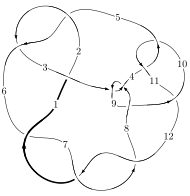
\includegraphics[width=112pt]{../../../GIT/diagram.site/Diagrams/png/1202_12a_0401.png}\\
\ \ \ A knot diagram\footnotemark}&
\allowdisplaybreaks
\textbf{Linearized knot diagam} \\
\cline{2-2}
 &
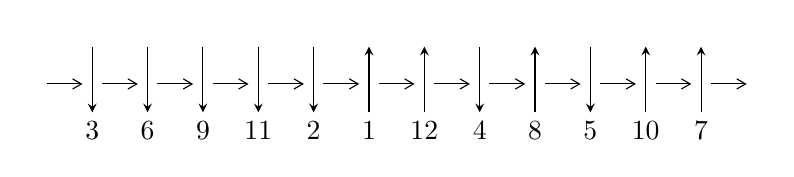
\begin{tikzpicture}[x=20pt, y=17pt]
	% nodes
	\node (C0) at (0, 0) {};
	\node (C1) at (1, 0) {};
	\node (C1U) at (1, +1) {};
	\node (C1D) at (1, -1) {3};

	\node (C2) at (2, 0) {};
	\node (C2U) at (2, +1) {};
	\node (C2D) at (2, -1) {6};

	\node (C3) at (3, 0) {};
	\node (C3U) at (3, +1) {};
	\node (C3D) at (3, -1) {9};

	\node (C4) at (4, 0) {};
	\node (C4U) at (4, +1) {};
	\node (C4D) at (4, -1) {11};

	\node (C5) at (5, 0) {};
	\node (C5U) at (5, +1) {};
	\node (C5D) at (5, -1) {2};

	\node (C6) at (6, 0) {};
	\node (C6U) at (6, +1) {};
	\node (C6D) at (6, -1) {1};

	\node (C7) at (7, 0) {};
	\node (C7U) at (7, +1) {};
	\node (C7D) at (7, -1) {12};

	\node (C8) at (8, 0) {};
	\node (C8U) at (8, +1) {};
	\node (C8D) at (8, -1) {4};

	\node (C9) at (9, 0) {};
	\node (C9U) at (9, +1) {};
	\node (C9D) at (9, -1) {8};

	\node (C10) at (10, 0) {};
	\node (C10U) at (10, +1) {};
	\node (C10D) at (10, -1) {5};

	\node (C11) at (11, 0) {};
	\node (C11U) at (11, +1) {};
	\node (C11D) at (11, -1) {10};

	\node (C12) at (12, 0) {};
	\node (C12U) at (12, +1) {};
	\node (C12D) at (12, -1) {7};
	\node (C13) at (13, 0) {};

	% arrows
	\draw[->,>={angle 60}]
	(C0) edge (C1) (C1) edge (C2) (C2) edge (C3) (C3) edge (C4) (C4) edge (C5) (C5) edge (C6) (C6) edge (C7) (C7) edge (C8) (C8) edge (C9) (C9) edge (C10) (C10) edge (C11) (C11) edge (C12) (C12) edge (C13) ;	\draw[->,>=stealth]
	(C1U) edge (C1D) (C2U) edge (C2D) (C3U) edge (C3D) (C4U) edge (C4D) (C5U) edge (C5D) (C6D) edge (C6U) (C7D) edge (C7U) (C8U) edge (C8D) (C9D) edge (C9U) (C10U) edge (C10D) (C11D) edge (C11U) (C12D) edge (C12U) ;
	\end{tikzpicture} \\
\hhline{~~} \\& 
\textbf{Solving Sequence} \\ \cline{2-2} 
 &
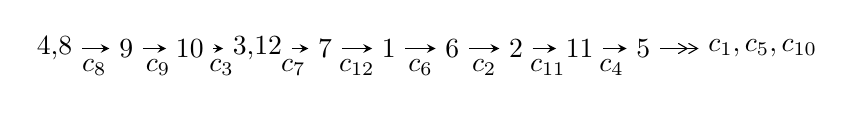
\begin{tikzpicture}[x=23pt, y=7pt]
	% node
	\node (A0) at (-1/8, 0) {4,8};
	\node (A1) at (1, 0) {9};
	\node (A2) at (2, 0) {10};
	\node (A3) at (49/16, 0) {3,12};
	\node (A4) at (33/8, 0) {7};
	\node (A5) at (41/8, 0) {1};
	\node (A6) at (49/8, 0) {6};
	\node (A7) at (57/8, 0) {2};
	\node (A8) at (65/8, 0) {11};
	\node (A9) at (73/8, 0) {5};
	\node (C1) at (1/2, -1) {$c_{8}$};
	\node (C2) at (3/2, -1) {$c_{9}$};
	\node (C3) at (5/2, -1) {$c_{3}$};
	\node (C4) at (29/8, -1) {$c_{7}$};
	\node (C5) at (37/8, -1) {$c_{12}$};
	\node (C6) at (45/8, -1) {$c_{6}$};
	\node (C7) at (53/8, -1) {$c_{2}$};
	\node (C8) at (61/8, -1) {$c_{11}$};
	\node (C9) at (69/8, -1) {$c_{4}$};
	\node (A10) at (11, 0) {$c_{1},c_{5},c_{10}$};

	% edge
	\draw[->,>=stealth]	
	(A0) edge (A1) (A1) edge (A2) (A2) edge (A3) (A3) edge (A4) (A4) edge (A5) (A5) edge (A6) (A6) edge (A7) (A7) edge (A8) (A8) edge (A9) ;
	\draw[->>,>={angle 60}]	
	(A9) edge (A10);
\end{tikzpicture} \\ 

\end{tabular} \\

\footnotetext{
The image of knot diagram is generated by the software ``\textbf{Draw programme}" developed by Andrew Bartholomew(\url{http://www.layer8.co.uk/maths/draw/index.htm\#Running-draw}), where we modified some parts for our purpose(\url{https://github.com/CATsTAILs/LinksPainter}).
}\phantom \\ \newline 
\centering \textbf{Ideals for irreducible components\footnotemark of $X_{\text{par}}$} 
 
\begin{align*}
I^u_{1}&=\langle 
u^{36}- u^{35}+\cdots+32 b+1,\;- u^4- u^2+a-1,\;u^{37}+7 u^{35}+\cdots+2 u-1\rangle \\
I^u_{2}&=\langle 
-3.61451\times10^{30} u^{51}-1.19611\times10^{30} u^{50}+\cdots+2.94109\times10^{31} b+1.36329\times10^{32},\\
\phantom{I^u_{2}}&\phantom{= \langle  }-4.07622\times10^{32} u^{51}-5.85781\times10^{32} u^{50}+\cdots+4.99985\times10^{32} a+2.17209\times10^{32},\\
\phantom{I^u_{2}}&\phantom{= \langle  }u^{52}+u^{51}+\cdots+30 u+17\rangle \\
I^u_{3}&=\langle 
b^5+b^4 u+2 b^3+b^2 u+b- u,\;a+1,\;u^2+1\rangle \\
\\
\end{align*}
\raggedright * 3 irreducible components of $\dim_{\mathbb{C}}=0$, with total 99 representations.\\
\footnotetext{All coefficients of polynomials are rational numbers. But the coefficients are sometimes approximated in decimal forms when there is not enough margin.}
\newpage
\renewcommand{\arraystretch}{1}
\centering \section*{I. $I^u_{1}= \langle u^{36}- u^{35}+\cdots+32 b+1,\;- u^4- u^2+a-1,\;u^{37}+7 u^{35}+\cdots+2 u-1 \rangle$}
\flushleft \textbf{(i) Arc colorings}\\
\begin{tabular}{m{7pt} m{180pt} m{7pt} m{180pt} }
\flushright $a_{4}=$&$\begin{pmatrix}0\\u\end{pmatrix}$ \\
\flushright $a_{8}=$&$\begin{pmatrix}1\\0\end{pmatrix}$ \\
\flushright $a_{9}=$&$\begin{pmatrix}1\\u^2\end{pmatrix}$ \\
\flushright $a_{10}=$&$\begin{pmatrix}u^2+1\\u^2\end{pmatrix}$ \\
\flushright $a_{3}=$&$\begin{pmatrix}u\\u^3+u\end{pmatrix}$ \\
\flushright $a_{12}=$&$\begin{pmatrix}u^4+u^2+1\\-0.0312500 u^{36}+0.0312500 u^{35}+\cdots+0.0937500 u-0.0312500\end{pmatrix}$ \\
\flushright $a_{7}=$&$\begin{pmatrix}-0.0312500 u^{36}+0.0312500 u^{35}+\cdots+0.0937500 u+0.968750\\0.343750 u^{36}-0.406250 u^{35}+\cdots-1.34375 u+0.468750\end{pmatrix}$ \\
\flushright $a_{1}=$&$\begin{pmatrix}\frac{1}{4} u^{36}-\frac{5}{16} u^{35}+\cdots-\frac{17}{16} u+\frac{11}{8}\\-0.812500 u^{36}+1.50000 u^{35}+\cdots+5.93750 u-2.25000\end{pmatrix}$ \\
\flushright $a_{6}=$&$\begin{pmatrix}-\frac{1}{8} u^{36}+\frac{5}{8} u^{35}+\cdots+\frac{47}{16} u-\frac{3}{16}\\-0.562500 u^{36}-1.37500 u^{35}+\cdots-8.62500 u+3.93750\end{pmatrix}$ \\
\flushright $a_{2}=$&$\begin{pmatrix}-\frac{1}{8} u^{36}+\frac{5}{8} u^{35}+\cdots+\frac{47}{16} u-\frac{3}{16}\\-\frac{19}{16} u^{36}+2 u^{35}+\cdots+\frac{123}{16} u-\frac{23}{8}\end{pmatrix}$ \\
\flushright $a_{11}=$&$\begin{pmatrix}1\\-0.0312500 u^{36}+0.0312500 u^{35}+\cdots+0.0937500 u-0.0312500\end{pmatrix}$ \\
\flushright $a_{5}=$&$\begin{pmatrix}- u\\-0.0312500 u^{36}-0.0312500 u^{35}+\cdots+0.968750 u+0.0312500\end{pmatrix}$\\&\end{tabular}
\flushleft \textbf{(ii) Obstruction class $= -1$}\\~\\
\flushleft \textbf{(iii) Cusp Shapes $= -\frac{67}{8} u^{36}-\frac{29}{8} u^{35}+\cdots-\frac{13}{4} u+\frac{19}{4}$}\\~\\
\newpage\renewcommand{\arraystretch}{1}
\flushleft \textbf{(iv) u-Polynomials at the component}\newline \\
\begin{tabular}{m{50pt}|m{274pt}}
Crossings & \hspace{64pt}u-Polynomials at each crossing \\
\hline $$\begin{aligned}c_{1}\end{aligned}$$&$\begin{aligned}
&u^{37}+21 u^{36}+\cdots-3 u+4
\end{aligned}$\\
\hline $$\begin{aligned}c_{2},c_{5}\end{aligned}$$&$\begin{aligned}
&u^{37}+3 u^{36}+\cdots+9 u+2
\end{aligned}$\\
\hline $$\begin{aligned}c_{3},c_{4},c_{8}\\c_{10}\end{aligned}$$&$\begin{aligned}
&u^{37}+7 u^{35}+\cdots+2 u+1
\end{aligned}$\\
\hline $$\begin{aligned}c_{6},c_{7},c_{12}\end{aligned}$$&$\begin{aligned}
&u^{37}+9 u^{36}+\cdots+251 u+22
\end{aligned}$\\
\hline $$\begin{aligned}c_{9},c_{11}\end{aligned}$$&$\begin{aligned}
&u^{37}-14 u^{36}+\cdots-10 u+1
\end{aligned}$\\
\hline
\end{tabular}\\~\\
\newpage\renewcommand{\arraystretch}{1}
\flushleft \textbf{(v) Riley Polynomials at the component}\newline \\
\begin{tabular}{m{50pt}|m{274pt}}
Crossings & \hspace{64pt}Riley Polynomials at each crossing \\
\hline $$\begin{aligned}c_{1}\end{aligned}$$&$\begin{aligned}
&y^{37}-9 y^{36}+\cdots+289 y-16
\end{aligned}$\\
\hline $$\begin{aligned}c_{2},c_{5}\end{aligned}$$&$\begin{aligned}
&y^{37}-21 y^{36}+\cdots-3 y-4
\end{aligned}$\\
\hline $$\begin{aligned}c_{3},c_{4},c_{8}\\c_{10}\end{aligned}$$&$\begin{aligned}
&y^{37}+14 y^{36}+\cdots-10 y-1
\end{aligned}$\\
\hline $$\begin{aligned}c_{6},c_{7},c_{12}\end{aligned}$$&$\begin{aligned}
&y^{37}+39 y^{36}+\cdots-1987 y-484
\end{aligned}$\\
\hline $$\begin{aligned}c_{9},c_{11}\end{aligned}$$&$\begin{aligned}
&y^{37}+30 y^{36}+\cdots+38 y-1
\end{aligned}$\\
\hline
\end{tabular}\\~\\
\newpage\flushleft \textbf{(vi) Complex Volumes and Cusp Shapes}
$$\begin{array}{c|c|c}  
\text{Solutions to }I^u_{1}& \I (\text{vol} + \sqrt{-1}CS) & \text{Cusp shape}\\
 \hline 
\begin{aligned}
u &= -0.670225 + 0.795123 I \\
a &= -0.285502 - 0.675689 I \\
b &= -0.008509 - 0.791858 I\end{aligned}
 & -4.22390 + 4.84801 I & -8.67350 - 6.63268 I \\ \hline\begin{aligned}
u &= -0.670225 - 0.795123 I \\
a &= -0.285502 + 0.675689 I \\
b &= -0.008509 + 0.791858 I\end{aligned}
 & -4.22390 - 4.84801 I & -8.67350 + 6.63268 I \\ \hline\begin{aligned}
u &= \phantom{-}0.480944 + 0.804131 I \\
a &= \phantom{-}0.158893 + 0.131000 I \\
b &= \phantom{-}0.330381 + 1.003000 I\end{aligned}
 & -0.56798 - 1.62654 I & -2.47163 + 4.05064 I \\ \hline\begin{aligned}
u &= \phantom{-}0.480944 - 0.804131 I \\
a &= \phantom{-}0.158893 - 0.131000 I \\
b &= \phantom{-}0.330381 - 1.003000 I\end{aligned}
 & -0.56798 + 1.62654 I & -2.47163 - 4.05064 I \\ \hline\begin{aligned}
u &= -0.885704 + 0.619459 I \\
a &= \phantom{-}0.35724 - 1.97679 I \\
b &= \phantom{-}0.07168 - 1.57263 I\end{aligned}
 & -8.61348 + 0.58442 I & -6.58298 - 2.11216 I \\ \hline\begin{aligned}
u &= -0.885704 - 0.619459 I \\
a &= \phantom{-}0.35724 + 1.97679 I \\
b &= \phantom{-}0.07168 + 1.57263 I\end{aligned}
 & -8.61348 - 0.58442 I & -6.58298 + 2.11216 I \\ \hline\begin{aligned}
u &= \phantom{-}0.906376 + 0.600235 I \\
a &= \phantom{-}0.49006 + 2.09180 I \\
b &= \phantom{-}0.14833 + 1.65936 I\end{aligned}
 & -12.33880 + 4.27785 I & -9.74358 - 1.05951 I \\ \hline\begin{aligned}
u &= \phantom{-}0.906376 - 0.600235 I \\
a &= \phantom{-}0.49006 - 2.09180 I \\
b &= \phantom{-}0.14833 - 1.65936 I\end{aligned}
 & -12.33880 - 4.27785 I & -9.74358 + 1.05951 I \\ \hline\begin{aligned}
u &= -0.378523 + 0.822123 I \\
a &= \phantom{-}0.363700 + 0.040587 I \\
b &= \phantom{-}0.35329 - 1.39171 I\end{aligned}
 & -3.60485 - 2.81236 I & -5.70776 - 1.61824 I \\ \hline\begin{aligned}
u &= -0.378523 - 0.822123 I \\
a &= \phantom{-}0.363700 - 0.040587 I \\
b &= \phantom{-}0.35329 + 1.39171 I\end{aligned}
 & -3.60485 + 2.81236 I & -5.70776 + 1.61824 I\\
 \hline 
 \end{array}$$\newpage$$\begin{array}{c|c|c}  
\text{Solutions to }I^u_{1}& \I (\text{vol} + \sqrt{-1}CS) & \text{Cusp shape}\\
 \hline 
\begin{aligned}
u &= \phantom{-}0.509957 + 0.977159 I \\
a &= -0.205307 - 0.388248 I \\
b &= \phantom{-}0.927591 + 0.449842 I\end{aligned}
 & \phantom{-}2.09312 - 1.88703 I & \phantom{-}0.31539 + 1.43334 I \\ \hline\begin{aligned}
u &= \phantom{-}0.509957 - 0.977159 I \\
a &= -0.205307 + 0.388248 I \\
b &= \phantom{-}0.927591 - 0.449842 I\end{aligned}
 & \phantom{-}2.09312 + 1.88703 I & \phantom{-}0.31539 - 1.43334 I \\ \hline\begin{aligned}
u &= \phantom{-}0.898488 + 0.646158 I \\
a &= \phantom{-}0.19345 + 2.06625 I \\
b &= -0.04381 + 1.61320 I\end{aligned}
 & -12.51130 - 5.32419 I & -9.84317 + 5.18460 I \\ \hline\begin{aligned}
u &= \phantom{-}0.898488 - 0.646158 I \\
a &= \phantom{-}0.19345 - 2.06625 I \\
b &= -0.04381 - 1.61320 I\end{aligned}
 & -12.51130 + 5.32419 I & -9.84317 - 5.18460 I \\ \hline\begin{aligned}
u &= -0.542969 + 1.023650 I \\
a &= -0.421670 + 0.562576 I \\
b &= \phantom{-}0.950468 - 0.040357 I\end{aligned}
 & \phantom{-}2.66475 + 6.19686 I & \phantom{-}1.89152 - 7.89879 I \\ \hline\begin{aligned}
u &= -0.542969 - 1.023650 I \\
a &= -0.421670 - 0.562576 I \\
b &= \phantom{-}0.950468 + 0.040357 I\end{aligned}
 & \phantom{-}2.66475 - 6.19686 I & \phantom{-}1.89152 + 7.89879 I \\ \hline\begin{aligned}
u &= -0.635272 + 0.460063 I \\
a &= \phantom{-}0.887068 - 0.808887 I \\
b &= \phantom{-}0.342500 - 0.887718 I\end{aligned}
 & -3.54036 - 2.08020 I & -9.14141 + 1.19821 I \\ \hline\begin{aligned}
u &= -0.635272 - 0.460063 I \\
a &= \phantom{-}0.887068 + 0.808887 I \\
b &= \phantom{-}0.342500 + 0.887718 I\end{aligned}
 & -3.54036 + 2.08020 I & -9.14141 - 1.19821 I \\ \hline\begin{aligned}
u &= \phantom{-}0.656373 + 1.034940 I \\
a &= -1.076160 - 0.381174 I \\
b &= \phantom{-}0.199892 - 0.364140 I\end{aligned}
 & -2.70237 - 5.71429 I & -7.25295 + 4.84897 I \\ \hline\begin{aligned}
u &= \phantom{-}0.656373 - 1.034940 I \\
a &= -1.076160 + 0.381174 I \\
b &= \phantom{-}0.199892 + 0.364140 I\end{aligned}
 & -2.70237 + 5.71429 I & -7.25295 - 4.84897 I\\
 \hline 
 \end{array}$$\newpage$$\begin{array}{c|c|c}  
\text{Solutions to }I^u_{1}& \I (\text{vol} + \sqrt{-1}CS) & \text{Cusp shape}\\
 \hline 
\begin{aligned}
u &= -0.290646 + 0.717353 I \\
a &= \phantom{-}0.581001 - 0.058279 I \\
b &= -0.274591 - 1.313790 I\end{aligned}
 & -3.81002 + 5.56820 I & -6.98582 - 8.76899 I \\ \hline\begin{aligned}
u &= -0.290646 - 0.717353 I \\
a &= \phantom{-}0.581001 + 0.058279 I \\
b &= -0.274591 + 1.313790 I\end{aligned}
 & -3.81002 - 5.56820 I & -6.98582 + 8.76899 I \\ \hline\begin{aligned}
u &= -0.593670 + 1.080170 I \\
a &= -0.796092 + 0.806284 I \\
b &= \phantom{-}0.797124 + 0.561418 I\end{aligned}
 & \phantom{-}1.77541 + 7.53533 I & \phantom{-}1.12920 - 6.50404 I \\ \hline\begin{aligned}
u &= -0.593670 - 1.080170 I \\
a &= -0.796092 - 0.806284 I \\
b &= \phantom{-}0.797124 - 0.561418 I\end{aligned}
 & \phantom{-}1.77541 - 7.53533 I & \phantom{-}1.12920 + 6.50404 I \\ \hline\begin{aligned}
u &= \phantom{-}0.607709 + 1.116880 I \\
a &= -0.949770 - 1.026550 I \\
b &= \phantom{-}0.797104 - 0.922482 I\end{aligned}
 & \phantom{-}0.06576 - 11.98300 I & -2.00000 + 11.09767 I \\ \hline\begin{aligned}
u &= \phantom{-}0.607709 - 1.116880 I \\
a &= -0.949770 + 1.026550 I \\
b &= \phantom{-}0.797104 + 0.922482 I\end{aligned}
 & \phantom{-}0.06576 + 11.98300 I & -2.00000 - 11.09767 I \\ \hline\begin{aligned}
u &= \phantom{-}0.358680 + 0.579084 I \\
a &= \phantom{-}0.663465 + 0.243691 I \\
b &= -0.108400 + 0.864333 I\end{aligned}
 & -0.64632 - 1.44283 I & -3.81239 + 5.10481 I \\ \hline\begin{aligned}
u &= \phantom{-}0.358680 - 0.579084 I \\
a &= \phantom{-}0.663465 - 0.243691 I \\
b &= -0.108400 - 0.864333 I\end{aligned}
 & -0.64632 + 1.44283 I & -3.81239 - 5.10481 I \\ \hline\begin{aligned}
u &= \phantom{-}0.675999 + 1.162370 I \\
a &= -1.56435 - 1.23880 I \\
b &= \phantom{-}0.24445 - 1.54342 I\end{aligned}
 & -5.08320 - 11.27570 I & -2.00000 + 6.81954 I \\ \hline\begin{aligned}
u &= \phantom{-}0.675999 - 1.162370 I \\
a &= -1.56435 + 1.23880 I \\
b &= \phantom{-}0.24445 + 1.54342 I\end{aligned}
 & -5.08320 + 11.27570 I & -2.00000 - 6.81954 I\\
 \hline 
 \end{array}$$\newpage$$\begin{array}{c|c|c}  
\text{Solutions to }I^u_{1}& \I (\text{vol} + \sqrt{-1}CS) & \text{Cusp shape}\\
 \hline 
\begin{aligned}
u &= -0.691615 + 1.157430 I \\
a &= -1.68262 + 1.15689 I \\
b &= \phantom{-}0.07127 + 1.51795 I\end{aligned}
 & -9.17720 + 6.73033 I & -6.31476 - 3.78221 I \\ \hline\begin{aligned}
u &= -0.691615 - 1.157430 I \\
a &= -1.68262 - 1.15689 I \\
b &= \phantom{-}0.07127 - 1.51795 I\end{aligned}
 & -9.17720 - 6.73033 I & -6.31476 + 3.78221 I \\ \hline\begin{aligned}
u &= -0.675732 + 1.175560 I \\
a &= -1.59314 + 1.35142 I \\
b &= \phantom{-}0.27313 + 1.68404 I\end{aligned}
 & -8.5942 + 16.2500 I & -5.34441 - 9.76292 I \\ \hline\begin{aligned}
u &= -0.675732 - 1.175560 I \\
a &= -1.59314 - 1.35142 I \\
b &= \phantom{-}0.27313 - 1.68404 I\end{aligned}
 & -8.5942 - 16.2500 I & -5.34441 + 9.76292 I \\ \hline\begin{aligned}
u &= \phantom{-}0.069180 + 0.547631 I \\
a &= \phantom{-}0.786237 + 0.031049 I \\
b &= -0.723577 + 0.256788 I\end{aligned}
 & \phantom{-}1.06858 - 1.83619 I & -0.74915 + 5.53995 I \\ \hline\begin{aligned}
u &= \phantom{-}0.069180 - 0.547631 I \\
a &= \phantom{-}0.786237 - 0.031049 I \\
b &= -0.723577 - 0.256788 I\end{aligned}
 & \phantom{-}1.06858 + 1.83619 I & -0.74915 - 5.53995 I \\ \hline\begin{aligned}
u &= \phantom{-}0.401304\phantom{ +0.000000I} \\
a &= \phantom{-}1.18698\phantom{ +0.000000I} \\
b &= \phantom{-}0.303349\phantom{ +0.000000I}\end{aligned}
 & -1.03663\phantom{ +0.000000I} & -10.7780\phantom{ +0.000000I}\\
 \hline 
 \end{array}$$\newpage\newpage\renewcommand{\arraystretch}{1}
\centering \section*{II. $I^u_{2}= \langle -3.61\times10^{30} u^{51}-1.20\times10^{30} u^{50}+\cdots+2.94\times10^{31} b+1.36\times10^{32},\;-4.08\times10^{32} u^{51}-5.86\times10^{32} u^{50}+\cdots+5.00\times10^{32} a+2.17\times10^{32},\;u^{52}+u^{51}+\cdots+30 u+17 \rangle$}
\flushleft \textbf{(i) Arc colorings}\\
\begin{tabular}{m{7pt} m{180pt} m{7pt} m{180pt} }
\flushright $a_{4}=$&$\begin{pmatrix}0\\u\end{pmatrix}$ \\
\flushright $a_{8}=$&$\begin{pmatrix}1\\0\end{pmatrix}$ \\
\flushright $a_{9}=$&$\begin{pmatrix}1\\u^2\end{pmatrix}$ \\
\flushright $a_{10}=$&$\begin{pmatrix}u^2+1\\u^2\end{pmatrix}$ \\
\flushright $a_{3}=$&$\begin{pmatrix}u\\u^3+u\end{pmatrix}$ \\
\flushright $a_{12}=$&$\begin{pmatrix}0.815268 u^{51}+1.17160 u^{50}+\cdots+23.9539 u-0.434432\\0.122897 u^{51}+0.0406690 u^{50}+\cdots-8.31341 u-4.63532\end{pmatrix}$ \\
\flushright $a_{7}=$&$\begin{pmatrix}-0.603660 u^{51}-0.550873 u^{50}+\cdots+5.39906 u+8.11570\\-0.0396776 u^{51}+0.142896 u^{50}+\cdots+13.1169 u+5.25900\end{pmatrix}$ \\
\flushright $a_{1}=$&$\begin{pmatrix}1.06030 u^{51}+0.970299 u^{50}+\cdots+4.31666 u-8.59212\\0.0653086 u^{51}-0.273432 u^{50}+\cdots-17.3837 u-7.10625\end{pmatrix}$ \\
\flushright $a_{6}=$&$\begin{pmatrix}-1.12011 u^{51}-0.813324 u^{50}+\cdots+13.6153 u+11.1311\\-0.0102037 u^{51}+0.271561 u^{50}+\cdots+24.6387 u+7.82138\end{pmatrix}$ \\
\flushright $a_{2}=$&$\begin{pmatrix}0.790972 u^{51}+0.764018 u^{50}+\cdots-5.28587 u-8.80006\\-0.262347 u^{51}-0.529752 u^{50}+\cdots-24.2991 u-8.38601\end{pmatrix}$ \\
\flushright $a_{11}=$&$\begin{pmatrix}0.580715 u^{51}+0.805430 u^{50}+\cdots+15.6537 u+0.380740\\-1\end{pmatrix}$ \\
\flushright $a_{5}=$&$\begin{pmatrix}0.165891 u^{51}+0.0542360 u^{50}+\cdots-24.5113 u-11.6369\\0.224715 u^{51}+0.113060 u^{50}+\cdots-16.0407 u-9.87216\end{pmatrix}$\\&\end{tabular}
\flushleft \textbf{(ii) Obstruction class $= -1$}\\~\\
\flushleft \textbf{(iii) Cusp Shapes $= 1.13196 u^{51}+1.65706 u^{50}+\cdots+16.1608 u-20.7826$}\\~\\
\newpage\renewcommand{\arraystretch}{1}
\flushleft \textbf{(iv) u-Polynomials at the component}\newline \\
\begin{tabular}{m{50pt}|m{274pt}}
Crossings & \hspace{64pt}u-Polynomials at each crossing \\
\hline $$\begin{aligned}c_{1}\end{aligned}$$&$\begin{aligned}
&(u^{26}+15 u^{25}+\cdots+3 u+1)^{2}
\end{aligned}$\\
\hline $$\begin{aligned}c_{2},c_{5}\end{aligned}$$&$\begin{aligned}
&(u^{26}- u^{25}+\cdots- u+1)^{2}
\end{aligned}$\\
\hline $$\begin{aligned}c_{3},c_{4},c_{8}\\c_{10}\end{aligned}$$&$\begin{aligned}
&u^{52}- u^{51}+\cdots-30 u+17
\end{aligned}$\\
\hline $$\begin{aligned}c_{6},c_{7},c_{12}\end{aligned}$$&$\begin{aligned}
&(u^{26}-3 u^{25}+\cdots-11 u+3)^{2}
\end{aligned}$\\
\hline $$\begin{aligned}c_{9},c_{11}\end{aligned}$$&$\begin{aligned}
&u^{52}-27 u^{51}+\cdots-3996 u+289
\end{aligned}$\\
\hline
\end{tabular}\\~\\
\newpage\renewcommand{\arraystretch}{1}
\flushleft \textbf{(v) Riley Polynomials at the component}\newline \\
\begin{tabular}{m{50pt}|m{274pt}}
Crossings & \hspace{64pt}Riley Polynomials at each crossing \\
\hline $$\begin{aligned}c_{1}\end{aligned}$$&$\begin{aligned}
&(y^{26}-7 y^{25}+\cdots+13 y+1)^{2}
\end{aligned}$\\
\hline $$\begin{aligned}c_{2},c_{5}\end{aligned}$$&$\begin{aligned}
&(y^{26}-15 y^{25}+\cdots-3 y+1)^{2}
\end{aligned}$\\
\hline $$\begin{aligned}c_{3},c_{4},c_{8}\\c_{10}\end{aligned}$$&$\begin{aligned}
&y^{52}+27 y^{51}+\cdots+3996 y+289
\end{aligned}$\\
\hline $$\begin{aligned}c_{6},c_{7},c_{12}\end{aligned}$$&$\begin{aligned}
&(y^{26}+29 y^{25}+\cdots+65 y+9)^{2}
\end{aligned}$\\
\hline $$\begin{aligned}c_{9},c_{11}\end{aligned}$$&$\begin{aligned}
&y^{52}-5 y^{51}+\cdots+1807796 y+83521
\end{aligned}$\\
\hline
\end{tabular}\\~\\
\newpage\flushleft \textbf{(vi) Complex Volumes and Cusp Shapes}
$$\begin{array}{c|c|c}  
\text{Solutions to }I^u_{2}& \I (\text{vol} + \sqrt{-1}CS) & \text{Cusp shape}\\
 \hline 
\begin{aligned}
u &= -0.550343 + 0.827493 I \\
a &= -1.93277 + 2.59907 I \\
b &= -0.09022 + 1.52061 I\end{aligned}
 & -4.80817 - 2.43962 I & -5.44223 + 0.17519 I \\ \hline\begin{aligned}
u &= -0.550343 - 0.827493 I \\
a &= -1.93277 - 2.59907 I \\
b &= -0.09022 - 1.52061 I\end{aligned}
 & -4.80817 + 2.43962 I & -5.44223 - 0.17519 I \\ \hline\begin{aligned}
u &= \phantom{-}0.529126 + 0.860647 I \\
a &= -1.71257 - 2.53937 I \\
b &= \phantom{-}0.08534 - 1.44303 I\end{aligned}
 & -1.01859 - 2.13264 I & -1.81035 + 3.16032 I \\ \hline\begin{aligned}
u &= \phantom{-}0.529126 - 0.860647 I \\
a &= -1.71257 + 2.53937 I \\
b &= \phantom{-}0.08534 + 1.44303 I\end{aligned}
 & -1.01859 + 2.13264 I & -1.81035 - 3.16032 I \\ \hline\begin{aligned}
u &= -0.554054 + 0.884455 I \\
a &= -1.61427 + 2.72347 I \\
b &= \phantom{-}0.19366 + 1.58163 I\end{aligned}
 & -4.61871 + 6.86486 I & -4.85861 - 6.16378 I \\ \hline\begin{aligned}
u &= -0.554054 - 0.884455 I \\
a &= -1.61427 - 2.72347 I \\
b &= \phantom{-}0.19366 - 1.58163 I\end{aligned}
 & -4.61871 - 6.86486 I & -4.85861 + 6.16378 I \\ \hline\begin{aligned}
u &= \phantom{-}0.951071 + 0.433551 I \\
a &= \phantom{-}0.04083 - 1.86805 I \\
b &= -0.17008 - 1.55712 I\end{aligned}
 & -7.30647 + 5.33673 I & -5.16942 - 2.96646 I \\ \hline\begin{aligned}
u &= \phantom{-}0.951071 - 0.433551 I \\
a &= \phantom{-}0.04083 + 1.86805 I \\
b &= -0.17008 + 1.55712 I\end{aligned}
 & -7.30647 - 5.33673 I & -5.16942 + 2.96646 I \\ \hline\begin{aligned}
u &= \phantom{-}0.764264 + 0.566838 I \\
a &= \phantom{-}0.607267 - 0.533028 I \\
b &= -0.087798 - 0.532774 I\end{aligned}
 & -4.08260 + 0.32949 I & -9.60033 + 0.20899 I \\ \hline\begin{aligned}
u &= \phantom{-}0.764264 - 0.566838 I \\
a &= \phantom{-}0.607267 + 0.533028 I \\
b &= -0.087798 + 0.532774 I\end{aligned}
 & -4.08260 - 0.32949 I & -9.60033 - 0.20899 I\\
 \hline 
 \end{array}$$\newpage$$\begin{array}{c|c|c}  
\text{Solutions to }I^u_{2}& \I (\text{vol} + \sqrt{-1}CS) & \text{Cusp shape}\\
 \hline 
\begin{aligned}
u &= -0.968590 + 0.418641 I \\
a &= -0.06346 + 2.01829 I \\
b &= -0.21971 + 1.67621 I\end{aligned}
 & -10.9094 - 10.2647 I & -8.13372 + 5.98641 I \\ \hline\begin{aligned}
u &= -0.968590 - 0.418641 I \\
a &= -0.06346 - 2.01829 I \\
b &= -0.21971 - 1.67621 I\end{aligned}
 & -10.9094 + 10.2647 I & -8.13372 - 5.98641 I \\ \hline\begin{aligned}
u &= \phantom{-}0.537250 + 0.915539 I \\
a &= \phantom{-}0.712664 + 0.797756 I \\
b &= -0.599592 + 0.613984 I\end{aligned}
 & -0.11782 - 2.56217 I & -2.00000 + 2.97329 I \\ \hline\begin{aligned}
u &= \phantom{-}0.537250 - 0.915539 I \\
a &= \phantom{-}0.712664 - 0.797756 I \\
b &= -0.599592 - 0.613984 I\end{aligned}
 & -0.11782 + 2.56217 I & -2.00000 - 2.97329 I \\ \hline\begin{aligned}
u &= -0.961357 + 0.458080 I \\
a &= \phantom{-}0.24305 + 1.92202 I \\
b &= -0.02106 + 1.56255 I\end{aligned}
 & -11.31370 - 0.70419 I & -8.80376 - 0.14810 I \\ \hline\begin{aligned}
u &= -0.961357 - 0.458080 I \\
a &= \phantom{-}0.24305 - 1.92202 I \\
b &= -0.02106 - 1.56255 I\end{aligned}
 & -11.31370 + 0.70419 I & -8.80376 + 0.14810 I \\ \hline\begin{aligned}
u &= \phantom{-}0.383435 + 0.995342 I \\
a &= -0.84645 - 1.77462 I \\
b &= \phantom{-}0.603458 - 0.686824 I\end{aligned}
 & \phantom{-}2.92792 - 3.85582 I & \phantom{-0.000000 -}0. + 7.89236 I \\ \hline\begin{aligned}
u &= \phantom{-}0.383435 - 0.995342 I \\
a &= -0.84645 + 1.77462 I \\
b &= \phantom{-}0.603458 + 0.686824 I\end{aligned}
 & \phantom{-}2.92792 + 3.85582 I & \phantom{-0.000000 } 0. - 7.89236 I \\ \hline\begin{aligned}
u &= -0.669360 + 0.847773 I \\
a &= \phantom{-}1.148410 - 0.546853 I \\
b &= -0.087798 - 0.532774 I\end{aligned}
 & -4.08260 + 0.32949 I & -9.60033 + 0.20899 I \\ \hline\begin{aligned}
u &= -0.669360 - 0.847773 I \\
a &= \phantom{-}1.148410 + 0.546853 I \\
b &= -0.087798 + 0.532774 I\end{aligned}
 & -4.08260 - 0.32949 I & -9.60033 - 0.20899 I\\
 \hline 
 \end{array}$$\newpage$$\begin{array}{c|c|c}  
\text{Solutions to }I^u_{2}& \I (\text{vol} + \sqrt{-1}CS) & \text{Cusp shape}\\
 \hline 
\begin{aligned}
u &= -0.284204 + 1.048140 I \\
a &= -0.627711 + 1.198740 I \\
b &= \phantom{-}0.559166 + 0.216872 I\end{aligned}
 & \phantom{-}4.34028 + 0.21572 I & \phantom{-}5.69812 - 1.13318 I \\ \hline\begin{aligned}
u &= -0.284204 - 1.048140 I \\
a &= -0.627711 - 1.198740 I \\
b &= \phantom{-}0.559166 - 0.216872 I\end{aligned}
 & \phantom{-}4.34028 - 0.21572 I & \phantom{-}5.69812 + 1.13318 I \\ \hline\begin{aligned}
u &= \phantom{-}0.786486 + 0.369460 I \\
a &= -0.422286 - 0.769115 I \\
b &= -0.648696 - 0.938364 I\end{aligned}
 & -2.10171 + 6.75127 I & -5.33497 - 7.43906 I \\ \hline\begin{aligned}
u &= \phantom{-}0.786486 - 0.369460 I \\
a &= -0.422286 + 0.769115 I \\
b &= -0.648696 + 0.938364 I\end{aligned}
 & -2.10171 - 6.75127 I & -5.33497 + 7.43906 I \\ \hline\begin{aligned}
u &= -0.577721 + 0.996615 I \\
a &= \phantom{-}0.768435 - 1.108730 I \\
b &= -0.648696 - 0.938364 I\end{aligned}
 & -2.10171 + 6.75127 I & -5.33497 - 7.43906 I \\ \hline\begin{aligned}
u &= -0.577721 - 0.996615 I \\
a &= \phantom{-}0.768435 + 1.108730 I \\
b &= -0.648696 + 0.938364 I\end{aligned}
 & -2.10171 - 6.75127 I & -5.33497 + 7.43906 I \\ \hline\begin{aligned}
u &= \phantom{-}0.342052 + 0.774444 I \\
a &= \phantom{-}0.464099 + 0.449574 I \\
b &= -0.791162 + 0.159676 I\end{aligned}
 & \phantom{-}1.10848 - 1.93104 I & -0.74595 + 4.18474 I \\ \hline\begin{aligned}
u &= \phantom{-}0.342052 - 0.774444 I \\
a &= \phantom{-}0.464099 - 0.449574 I \\
b &= -0.791162 - 0.159676 I\end{aligned}
 & \phantom{-}1.10848 + 1.93104 I & -0.74595 - 4.18474 I \\ \hline\begin{aligned}
u &= -0.224633 + 1.133270 I \\
a &= -0.300749 + 0.796598 I \\
b &= \phantom{-}0.559166 - 0.216872 I\end{aligned}
 & \phantom{-}4.34028 - 0.21572 I & \phantom{-}5.69812 + 0. I\phantom{ +0.000000I} \\ \hline\begin{aligned}
u &= -0.224633 - 1.133270 I \\
a &= -0.300749 - 0.796598 I \\
b &= \phantom{-}0.559166 + 0.216872 I\end{aligned}
 & \phantom{-}4.34028 + 0.21572 I & \phantom{-}5.69812 + 0. I\phantom{ +0.000000I}\\
 \hline 
 \end{array}$$\newpage$$\begin{array}{c|c|c}  
\text{Solutions to }I^u_{2}& \I (\text{vol} + \sqrt{-1}CS) & \text{Cusp shape}\\
 \hline 
\begin{aligned}
u &= \phantom{-}0.036728 + 1.177540 I \\
a &= -0.397670 - 0.124485 I \\
b &= -0.313295 + 0.402304 I\end{aligned}
 & \phantom{-}1.71189 - 1.00473 I & -5.82896 + 0. I\phantom{ +0.000000I} \\ \hline\begin{aligned}
u &= \phantom{-}0.036728 - 1.177540 I \\
a &= -0.397670 + 0.124485 I \\
b &= -0.313295 - 0.402304 I\end{aligned}
 & \phantom{-}1.71189 + 1.00473 I & -5.82896 + 0. I\phantom{ +0.000000I} \\ \hline\begin{aligned}
u &= -0.690243 + 0.417206 I \\
a &= -0.132047 + 0.281676 I \\
b &= -0.599592 + 0.613984 I\end{aligned}
 & -0.11782 - 2.56217 I & -1.94700 + 2.97329 I \\ \hline\begin{aligned}
u &= -0.690243 - 0.417206 I \\
a &= -0.132047 - 0.281676 I \\
b &= -0.599592 - 0.613984 I\end{aligned}
 & -0.11782 + 2.56217 I & -1.94700 - 2.97329 I \\ \hline\begin{aligned}
u &= \phantom{-}0.203821 + 1.221330 I \\
a &= \phantom{-}0.017866 - 0.514233 I \\
b &= \phantom{-}0.603458 + 0.686824 I\end{aligned}
 & \phantom{-}2.92792 + 3.85582 I & \phantom{-0.000000 } 0 \\ \hline\begin{aligned}
u &= \phantom{-}0.203821 - 1.221330 I \\
a &= \phantom{-}0.017866 + 0.514233 I \\
b &= \phantom{-}0.603458 - 0.686824 I\end{aligned}
 & \phantom{-}2.92792 - 3.85582 I & \phantom{-0.000000 } 0 \\ \hline\begin{aligned}
u &= \phantom{-}0.220997 + 0.724279 I \\
a &= -2.17171 - 0.98902 I \\
b &= -0.313295 - 0.402304 I\end{aligned}
 & \phantom{-}1.71189 + 1.00473 I & -5.82896 - 0.57498 I \\ \hline\begin{aligned}
u &= \phantom{-}0.220997 - 0.724279 I \\
a &= -2.17171 + 0.98902 I \\
b &= -0.313295 + 0.402304 I\end{aligned}
 & \phantom{-}1.71189 - 1.00473 I & -5.82896 + 0.57498 I \\ \hline\begin{aligned}
u &= -0.720229 + 1.047070 I \\
a &= \phantom{-}1.40344 - 1.54237 I \\
b &= -0.17008 - 1.55712 I\end{aligned}
 & -7.30647 + 5.33673 I & \phantom{-0.000000 } 0 \\ \hline\begin{aligned}
u &= -0.720229 - 1.047070 I \\
a &= \phantom{-}1.40344 + 1.54237 I \\
b &= -0.17008 + 1.55712 I\end{aligned}
 & -7.30647 - 5.33673 I & \phantom{-0.000000 } 0\\
 \hline 
 \end{array}$$\newpage$$\begin{array}{c|c|c}  
\text{Solutions to }I^u_{2}& \I (\text{vol} + \sqrt{-1}CS) & \text{Cusp shape}\\
 \hline 
\begin{aligned}
u &= \phantom{-}0.741481 + 1.037370 I \\
a &= \phantom{-}1.54716 + 1.50406 I \\
b &= -0.02106 + 1.56255 I\end{aligned}
 & -11.31370 - 0.70419 I & \phantom{-0.000000 } 0 \\ \hline\begin{aligned}
u &= \phantom{-}0.741481 - 1.037370 I \\
a &= \phantom{-}1.54716 - 1.50406 I \\
b &= -0.02106 - 1.56255 I\end{aligned}
 & -11.31370 + 0.70419 I & \phantom{-0.000000 } 0 \\ \hline\begin{aligned}
u &= \phantom{-}0.722575 + 1.066990 I \\
a &= \phantom{-}1.39072 + 1.66975 I \\
b &= -0.21971 + 1.67621 I\end{aligned}
 & -10.9094 - 10.2647 I & \phantom{-0.000000 } 0 \\ \hline\begin{aligned}
u &= \phantom{-}0.722575 - 1.066990 I \\
a &= \phantom{-}1.39072 - 1.66975 I \\
b &= -0.21971 - 1.67621 I\end{aligned}
 & -10.9094 + 10.2647 I & \phantom{-0.000000 } 0 \\ \hline\begin{aligned}
u &= \phantom{-}0.117241 + 1.324870 I \\
a &= \phantom{-}0.0151086 + 0.0789385 I \\
b &= \phantom{-}0.08534 + 1.44303 I\end{aligned}
 & -1.01859 + 2.13264 I & \phantom{-0.000000 } 0 \\ \hline\begin{aligned}
u &= \phantom{-}0.117241 - 1.324870 I \\
a &= \phantom{-}0.0151086 - 0.0789385 I \\
b &= \phantom{-}0.08534 - 1.44303 I\end{aligned}
 & -1.01859 - 2.13264 I & \phantom{-0.000000 } 0 \\ \hline\begin{aligned}
u &= -0.095137 + 1.336100 I \\
a &= -0.059114 - 0.156098 I \\
b &= -0.09022 - 1.52061 I\end{aligned}
 & -4.80817 + 2.43962 I & \phantom{-0.000000 } 0 \\ \hline\begin{aligned}
u &= -0.095137 - 1.336100 I \\
a &= -0.059114 + 0.156098 I \\
b &= -0.09022 + 1.52061 I\end{aligned}
 & -4.80817 - 2.43962 I & \phantom{-0.000000 } 0 \\ \hline\begin{aligned}
u &= -0.131274 + 1.342360 I \\
a &= \phantom{-}0.105716 - 0.128904 I \\
b &= \phantom{-}0.19366 - 1.58163 I\end{aligned}
 & -4.61871 - 6.86486 I & \phantom{-0.000000 } 0 \\ \hline\begin{aligned}
u &= -0.131274 - 1.342360 I \\
a &= \phantom{-}0.105716 + 0.128904 I \\
b &= \phantom{-}0.19366 + 1.58163 I\end{aligned}
 & -4.61871 + 6.86486 I & \phantom{-0.000000 } 0\\
 \hline 
 \end{array}$$\newpage$$\begin{array}{c|c|c}  
\text{Solutions to }I^u_{2}& \I (\text{vol} + \sqrt{-1}CS) & \text{Cusp shape}\\
 \hline 
\begin{aligned}
u &= -0.409385 + 0.446289 I \\
a &= \phantom{-}0.286631 - 0.591162 I \\
b &= -0.791162 + 0.159676 I\end{aligned}
 & \phantom{-}1.10848 - 1.93104 I & -0.74595 + 4.18474 I \\ \hline\begin{aligned}
u &= -0.409385 - 0.446289 I \\
a &= \phantom{-}0.286631 + 0.591162 I \\
b &= -0.791162 - 0.159676 I\end{aligned}
 & \phantom{-}1.10848 + 1.93104 I & -0.74595 - 4.18474 I\\
 \hline 
 \end{array}$$\newpage\newpage\renewcommand{\arraystretch}{1}
\centering \section*{III. $I^u_{3}= \langle b^5+b^4 u+2 b^3+b^2 u+b- u,\;a+1,\;u^2+1 \rangle$}
\flushleft \textbf{(i) Arc colorings}\\
\begin{tabular}{m{7pt} m{180pt} m{7pt} m{180pt} }
\flushright $a_{4}=$&$\begin{pmatrix}0\\u\end{pmatrix}$ \\
\flushright $a_{8}=$&$\begin{pmatrix}1\\0\end{pmatrix}$ \\
\flushright $a_{9}=$&$\begin{pmatrix}1\\-1\end{pmatrix}$ \\
\flushright $a_{10}=$&$\begin{pmatrix}0\\-1\end{pmatrix}$ \\
\flushright $a_{3}=$&$\begin{pmatrix}u\\0\end{pmatrix}$ \\
\flushright $a_{12}=$&$\begin{pmatrix}-1\\b\end{pmatrix}$ \\
\flushright $a_{7}=$&$\begin{pmatrix}- b+1\\b^2\end{pmatrix}$ \\
\flushright $a_{1}=$&$\begin{pmatrix}- b^2+b-1\\b^3+b\end{pmatrix}$ \\
\flushright $a_{6}=$&$\begin{pmatrix}- b^3+b^2-2 b+1\\b^4+2 b^2\end{pmatrix}$ \\
\flushright $a_{2}=$&$\begin{pmatrix}b^3- b^2+2 b-1\\b^3+b\end{pmatrix}$ \\
\flushright $a_{11}=$&$\begin{pmatrix}-1\\b-1\end{pmatrix}$ \\
\flushright $a_{5}=$&$\begin{pmatrix}- u\\b u\end{pmatrix}$\\&\end{tabular}
\flushleft \textbf{(ii) Obstruction class $= 1$}\\~\\
\flushleft \textbf{(iii) Cusp Shapes $= -4 b^3 u-8 b u$}\\~\\
\newpage\renewcommand{\arraystretch}{1}
\flushleft \textbf{(iv) u-Polynomials at the component}\newline \\
\begin{tabular}{m{50pt}|m{274pt}}
Crossings & \hspace{64pt}u-Polynomials at each crossing \\
\hline $$\begin{aligned}c_{1}\end{aligned}$$&$\begin{aligned}
&(u^5-3 u^4+4 u^3- u^2- u+1)^2
\end{aligned}$\\
\hline $$\begin{aligned}c_{2},c_{5}\end{aligned}$$&$\begin{aligned}
&u^{10}-3 u^8+4 u^6- u^4- u^2+1
\end{aligned}$\\
\hline $$\begin{aligned}c_{3},c_{4},c_{8}\\c_{10}\end{aligned}$$&$\begin{aligned}
&(u^2+1)^5
\end{aligned}$\\
\hline $$\begin{aligned}c_{6},c_{7},c_{12}\end{aligned}$$&$\begin{aligned}
&u^{10}+5 u^8+8 u^6+3 u^4- u^2+1
\end{aligned}$\\
\hline $$\begin{aligned}c_{9},c_{11}\end{aligned}$$&$\begin{aligned}
&(u-1)^{10}
\end{aligned}$\\
\hline
\end{tabular}\\~\\
\newpage\renewcommand{\arraystretch}{1}
\flushleft \textbf{(v) Riley Polynomials at the component}\newline \\
\begin{tabular}{m{50pt}|m{274pt}}
Crossings & \hspace{64pt}Riley Polynomials at each crossing \\
\hline $$\begin{aligned}c_{1}\end{aligned}$$&$\begin{aligned}
&(y^5- y^4+8 y^3-3 y^2+3 y-1)^2
\end{aligned}$\\
\hline $$\begin{aligned}c_{2},c_{5}\end{aligned}$$&$\begin{aligned}
&(y^5-3 y^4+4 y^3- y^2- y+1)^2
\end{aligned}$\\
\hline $$\begin{aligned}c_{3},c_{4},c_{8}\\c_{10}\end{aligned}$$&$\begin{aligned}
&(y+1)^{10}
\end{aligned}$\\
\hline $$\begin{aligned}c_{6},c_{7},c_{12}\end{aligned}$$&$\begin{aligned}
&(y^5+5 y^4+8 y^3+3 y^2- y+1)^2
\end{aligned}$\\
\hline $$\begin{aligned}c_{9},c_{11}\end{aligned}$$&$\begin{aligned}
&(y-1)^{10}
\end{aligned}$\\
\hline
\end{tabular}\\~\\
\newpage\flushleft \textbf{(vi) Complex Volumes and Cusp Shapes}
$$\begin{array}{c|c|c}  
\text{Solutions to }I^u_{3}& \I (\text{vol} + \sqrt{-1}CS) & \text{Cusp shape}\\
 \hline 
\begin{aligned}
u &= \phantom{-0.000000 -}1.000000 I \\
a &= -1.00000\phantom{ +0.000000I} \\
b &= \phantom{-0.000000 -}1.217740 I\end{aligned}
 & \phantom{-}0.888787\phantom{ +0.000000I} & \phantom{-}2.51890\phantom{ +0.000000I} \\ \hline\begin{aligned}
u &= \phantom{-0.000000 -}1.000000 I \\
a &= -1.00000\phantom{ +0.000000I} \\
b &= \phantom{-}0.549911 + 0.309916 I\end{aligned}
 & \phantom{-}2.96077 + 1.53058 I & \phantom{-}3.48489 - 4.43065 I \\ \hline\begin{aligned}
u &= \phantom{-0.000000 -}1.000000 I \\
a &= -1.00000\phantom{ +0.000000I} \\
b &= -0.549911 + 0.309916 I\end{aligned}
 & \phantom{-}2.96077 - 1.53058 I & \phantom{-}3.48489 + 4.43065 I \\ \hline\begin{aligned}
u &= \phantom{-0.000000 -}1.000000 I \\
a &= -1.00000\phantom{ +0.000000I} \\
b &= \phantom{-}0.21917 - 1.41878 I\end{aligned}
 & -2.58269 - 4.40083 I & -0.74431 + 3.49859 I \\ \hline\begin{aligned}
u &= \phantom{-0.000000 -}1.000000 I \\
a &= -1.00000\phantom{ +0.000000I} \\
b &= -0.21917 - 1.41878 I\end{aligned}
 & -2.58269 + 4.40083 I & -0.74431 - 3.49859 I \\ \hline\begin{aligned}
u &= \phantom{-0.000000 } -1.000000 I \\
a &= -1.00000\phantom{ +0.000000I} \\
b &= \phantom{-0.000000 } -1.217740 I\end{aligned}
 & \phantom{-}0.888787\phantom{ +0.000000I} & \phantom{-}2.51890\phantom{ +0.000000I} \\ \hline\begin{aligned}
u &= \phantom{-0.000000 } -1.000000 I \\
a &= -1.00000\phantom{ +0.000000I} \\
b &= \phantom{-}0.549911 - 0.309916 I\end{aligned}
 & \phantom{-}2.96077 - 1.53058 I & \phantom{-}3.48489 + 4.43065 I \\ \hline\begin{aligned}
u &= \phantom{-0.000000 } -1.000000 I \\
a &= -1.00000\phantom{ +0.000000I} \\
b &= -0.549911 - 0.309916 I\end{aligned}
 & \phantom{-}2.96077 + 1.53058 I & \phantom{-}3.48489 - 4.43065 I \\ \hline\begin{aligned}
u &= \phantom{-0.000000 } -1.000000 I \\
a &= -1.00000\phantom{ +0.000000I} \\
b &= -0.21917 + 1.41878 I\end{aligned}
 & -2.58269 + 4.40083 I & -0.74431 - 3.49859 I \\ \hline\begin{aligned}
u &= \phantom{-0.000000 } -1.000000 I \\
a &= -1.00000\phantom{ +0.000000I} \\
b &= \phantom{-}0.21917 + 1.41878 I\end{aligned}
 & -2.58269 - 4.40083 I & -0.74431 + 3.49859 I\\
 \hline 
 \end{array}$$\newpage
\newpage\renewcommand{\arraystretch}{1}
\centering \section*{ IV. u-Polynomials}
\begin{tabular}{m{50pt}|m{274pt}}
Crossings & \hspace{64pt}u-Polynomials at each crossing \\
\hline $$\begin{aligned}c_{1}\end{aligned}$$&$\begin{aligned}
&((u^5-3 u^4+4 u^3- u^2- u+1)^2)(u^{26}+15 u^{25}+\cdots+3 u+1)^{2}\\
&\cdot(u^{37}+21 u^{36}+\cdots-3 u+4)
\end{aligned}$\\
\hline $$\begin{aligned}c_{2},c_{5}\end{aligned}$$&$\begin{aligned}
&(u^{10}-3 u^8+4 u^6- u^4- u^2+1)(u^{26}- u^{25}+\cdots- u+1)^{2}\\
&\cdot(u^{37}+3 u^{36}+\cdots+9 u+2)
\end{aligned}$\\
\hline $$\begin{aligned}c_{3},c_{4},c_{8}\\c_{10}\end{aligned}$$&$\begin{aligned}
&((u^2+1)^5)(u^{37}+7 u^{35}+\cdots+2 u+1)(u^{52}- u^{51}+\cdots-30 u+17)
\end{aligned}$\\
\hline $$\begin{aligned}c_{6},c_{7},c_{12}\end{aligned}$$&$\begin{aligned}
&(u^{10}+5 u^8+8 u^6+3 u^4- u^2+1)(u^{26}-3 u^{25}+\cdots-11 u+3)^{2}\\
&\cdot(u^{37}+9 u^{36}+\cdots+251 u+22)
\end{aligned}$\\
\hline $$\begin{aligned}c_{9},c_{11}\end{aligned}$$&$\begin{aligned}
&((u-1)^{10})(u^{37}-14 u^{36}+\cdots-10 u+1)\\
&\cdot(u^{52}-27 u^{51}+\cdots-3996 u+289)
\end{aligned}$\\
\hline
\end{tabular}\newpage\renewcommand{\arraystretch}{1}
\centering \section*{ V. Riley Polynomials}
\begin{tabular}{m{50pt}|m{274pt}}
Crossings & \hspace{64pt}Riley Polynomials at each crossing \\
\hline $$\begin{aligned}c_{1}\end{aligned}$$&$\begin{aligned}
&((y^5- y^4+8 y^3-3 y^2+3 y-1)^2)(y^{26}-7 y^{25}+\cdots+13 y+1)^{2}\\
&\cdot(y^{37}-9 y^{36}+\cdots+289 y-16)
\end{aligned}$\\
\hline $$\begin{aligned}c_{2},c_{5}\end{aligned}$$&$\begin{aligned}
&((y^5-3 y^4+4 y^3- y^2- y+1)^2)(y^{26}-15 y^{25}+\cdots-3 y+1)^{2}\\
&\cdot(y^{37}-21 y^{36}+\cdots-3 y-4)
\end{aligned}$\\
\hline $$\begin{aligned}c_{3},c_{4},c_{8}\\c_{10}\end{aligned}$$&$\begin{aligned}
&((y+1)^{10})(y^{37}+14 y^{36}+\cdots-10 y-1)\\
&\cdot(y^{52}+27 y^{51}+\cdots+3996 y+289)
\end{aligned}$\\
\hline $$\begin{aligned}c_{6},c_{7},c_{12}\end{aligned}$$&$\begin{aligned}
&((y^5+5 y^4+8 y^3+3 y^2- y+1)^2)(y^{26}+29 y^{25}+\cdots+65 y+9)^{2}\\
&\cdot(y^{37}+39 y^{36}+\cdots-1987 y-484)
\end{aligned}$\\
\hline $$\begin{aligned}c_{9},c_{11}\end{aligned}$$&$\begin{aligned}
&((y-1)^{10})(y^{37}+30 y^{36}+\cdots+38 y-1)\\
&\cdot(y^{52}-5 y^{51}+\cdots+1807796 y+83521)
\end{aligned}$\\
\hline
\end{tabular}
\vskip 2pc
\end{document}